\chapter{Improvements}{\label{chap:Improvements}
Multiple ideas were applied to improve the performance of baseline, PARSEC \cite{PARSEC_VD}.
This chapter lists each idea and its individual impact on performance.
All improvements are then combined to present final results in Chapter \ref{chap:Results}.
The basic philosophy used is to find the most time-consuming step and try to make it faster using algorithmic or computational techniques.

The criteria used for quantifying the contributions of these improvements are number of intersections and runtime.
These numbers are reported as speedups, the ratio of old to new.
Formally, we define the intersection speedup and time speedup as:
$$
    \text{Intersection Speedup} = \frac{\text{\# of Intersections Baseline}}{\text{\# of Intersections New}}
$$
$$
    \text{Time Speedup} = \frac{\text{Run time Baseline}}{\text{Run time New}}
$$
The information of data graphs and queries used to report individual performance impact is mentioned in Section \ref{sec:expt-info}.

\section{Intersection Reuse}\label{sec:reuse-impl}
Set intersection operation for generating candidates at the next level is the most time-consuming operation in subgraph enumeration, this is a well-established fact in the literature \cite{RPS-paper}, \cite{LIGHT}, \cite{VF3}.
This was also verified for the baseline \cite{PARSEC_VD}. Figure \ref{fig:time-dist} gives the distribution of time spent by each operation in different tasks. The Intersect operation shown here is the time taken by Algorithm \ref{algo:intersect}.
\begin{figure}
    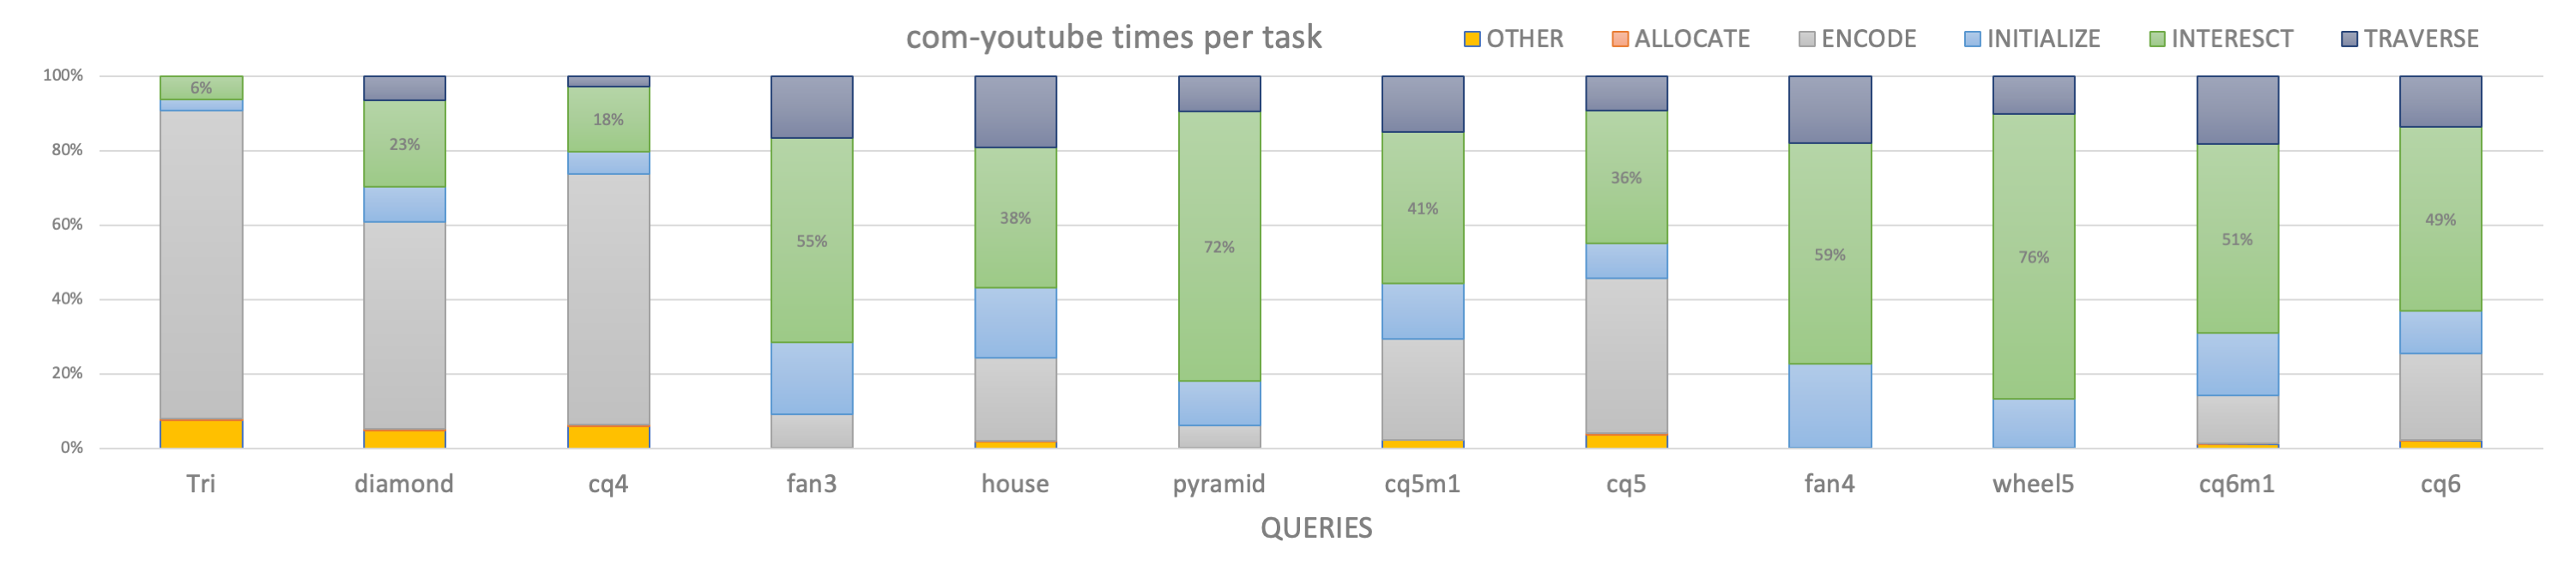
\includegraphics[width=\textwidth]{fig/improvements/time-distributions-yt.png}
    \caption{Stepwise Fraction Time spent}
    \label{fig:time-dist}
\end{figure}
This algorithm involves iterating over each element of the backward element list to perform intersection and generate possible candidates for next level (lines 2 - 5).
The number of backward neighbors at each level increases with increasing template size. This results in even more adjacency list intersections at each node.
RPS \cite{RPS-paper} reduces these operations by generating an intersection reuse plan, this plan smartly finds the intersections that will be required by more than one node and stores them when first calculated. There is a lot of intersection reuse possible with RPS as they employ a BFS strategy.
Similar extent of reuse is not possible in DFS traversal since the past information is lost while backtracking.
However, Some levels of the sequenced query graphs have similar backward neighbor lists. For such queries, the majority of intersections can be reused by simply storing the intermediate intersection results.
To do this efficiently, one needs to match levels with similar adjacency lists. This problem is posed as a linear programming optimization problem.

Let, the sequenced query graph be $G_q=(V_q, E_q)$ with $|V_q|=k$ and the vertex sequence $S_q$.
$\mathcal{N}(.)$ be the function for getting the backward neighbor list of a vertex.
For each pair of vertices at level $i$ and $j$ let $W_{ij}$ be a measure of the commonality between their backward neighbors'. Let $X_{i,j}$ be the decision variable which tells if vertex $i$ should reuse intersections from vertex $j$.

With these definitions the optimization problem can be modelled as:
\begin{align}
    \max \sum_{i=j+1}^{k}\sum_{j=1}^{k} W_{ij} X_{ij} \\
    \text{s.t.}
    \sum_{j=1}^k X_{ij} \leq 1. \quad \forall i \in \{1, \dots, k\}
\end{align}
Where, $$
    W_{ij} = \begin{cases}
        |\mathcal{N}(S_q[i]) \cap \mathcal{N}(S_q[j])| \qquad \text{if} \quad i>j, \mathcal{N}(S_q[i]) \supseteq \mathcal{N}(S_q[j]) \\
        0   \qquad \text{Otherwise}
    \end{cases}
$$
This problem is a linear semi-assignment problem (LSAP) where the greedy solution is optimal.
% This is easy to establish as any other solution can be improved by switching to the ÷greedy solution.
The solution to this problem is:
$$
    X_{ij}=\begin{cases}
        1   \qquad \text{if } j=\argmax_j(w_{ij}>0); \\
        0   \qquad \text{Otherwise}
    \end{cases}
$$
Reuse detection involves a find minimum operation for each level in $G_q$ hence it is polynomial time and can be performed on CPU for small-sized query graphs.
The mappings found $x_{ij} = 1$ implies that level $i$ can use intersection results from level $j$.
Hence, the level $j$ is flagged as \textit{reusable} and its results are stored along with the DFS stack.
Algorithm \ref{algo:reuse} lists the reuse detection and post-processing recipe.
To save on constant memory the query graphs are stored in CSR format.
After finding the reuse mappings from the query, the column index of $(G_q)$ needs to be modified for the search tree traversal step to utilize this information.
The modification step involves reordering the lists and generating the reuse pointer array.

We show reuse detection at work on the example query in Figure \ref{fig:sgm-example}.
Here, only $w_{54}$ and $w_{53}$ are positive with value 2. Hence, any of the levels 3 or 4 can be marked reusable, Let's assume level 4.
The backward neighbors of level four are $\{1,3\}$ and for level five they are $\{1,2,3\}$. To avoid checks in the for loop of Algorithm \ref{algo:intersect} (line 2).
Another Reuse pointer array is created which gives the start of the remaining neighbors of level 5.

\begin{figure}
    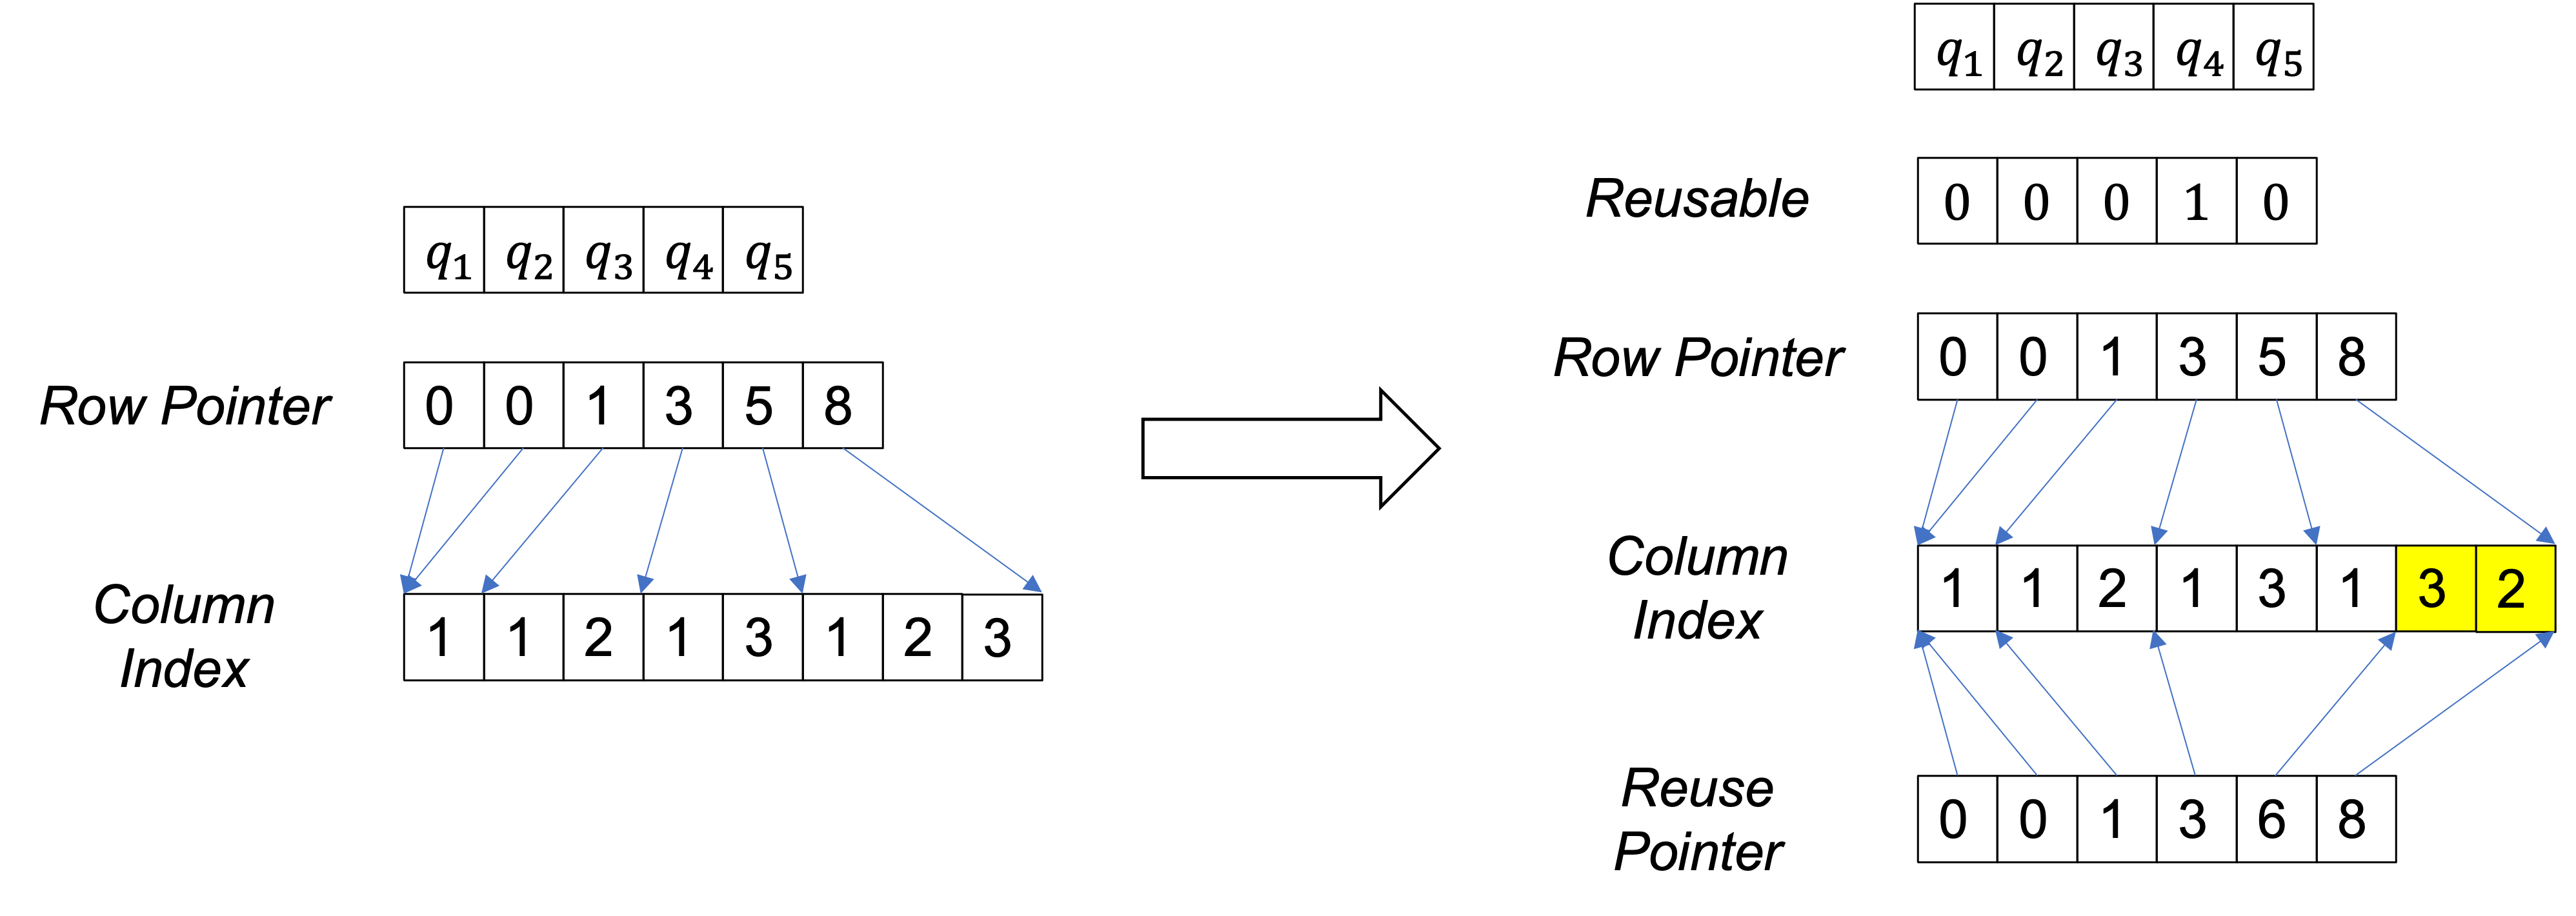
\includegraphics[width=\textwidth]{fig/improvements/Reuse-resorting.png}
    \caption{Reuse Detection Example}
    \label{fig:reuse-detection}
\end{figure}
Once the reuse is detected and pointers set, this data is sent to the GPU constant memory for the rest of the application. For implementing reuse, the function in Algorithm \ref{algo:intersect} needs to be changed to add conditions for checking if a level is reusable or if the reuse pointer is updated. This is shown as a flow chart in Figure \ref{fig:reuse-flowchart}.
\begin{figure}
    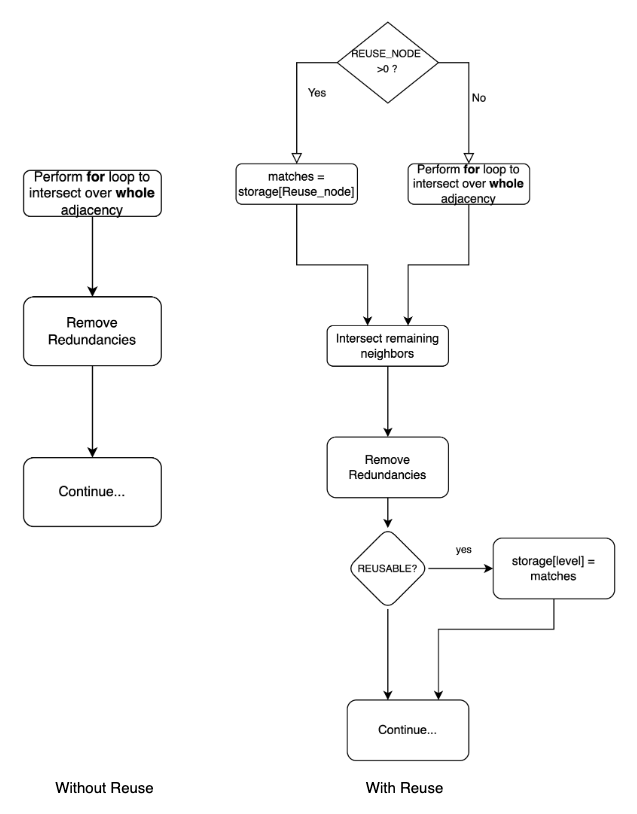
\includegraphics[width=\textwidth]{fig/improvements/reuse-flow.png}
    \caption{Flowchart with and without reuse}
    \label{fig:reuse-flowchart}
\end{figure}
This way, reuse reduces computational workload and adds to the memory workload.
Since global memory writes are relatively expensive, some shared memory can be utilized to write the intermediate intersection results while longer results can be spilled to global memory.

\begin{algorithm}
    \caption{Reuse Detection}
    \label{algo:reuse}
    \SetKwData{qgraph}{$G_q=(V_q, E_q)$}
    \SetKwData{bneighbor}{$\mathcal{N}(V_q)$}
    \SetKwData{reusable}{$\texttt{reusable}$}
    \KwIn{Directed Query Graph \qgraph \newline
        Arrray of Backward Neighbor lists \bneighbor
    }
    $W \leftarrow: [|V_q|][|V_q|]$\;
    $X \leftarrow: [|V_q|][|V_q|]$\;
    \reusable $\leftarrow: [|V_q|]$\;
    \ForAll{$j \in V_q$}{
        \For{$i=j+1 \textbf{ to } |V_q|$}{
            \leIf{$\bneighbor[i] \supseteq \bneighbor[j]$}{
                $W[i][j] \leftarrow |\bneighbor[i] \cap \bneighbor[j]|$\;
            }
            {
                $W[i][j] \leftarrow 0$
            }
        }
    }
    $\reusable[j] \leftarrow (\max({W[i].)} > 0)$\;
    \ForAll{$i \in V_q$}{
        \For{$j=1 \textbf{ to } i$}{
            \leIf(){$j==\argmax_j(W[i]. > 0)$}{$1$\; $\reusable[j]=1$\;}{0}
        }
    }
    \CommentSty{\texttt{// Update Reuse Pointers from $X[i][j]$}}
\end{algorithm}

The improvements due to intersection reuse are measured in terms of the number of intersections performed.
Since there are increased reads and writes to global memory the time benefit from this technique is negligible. Table \ref{tab:reuse-improvement} shows the improvement in the number of intersections with this technique.
Since the backward neighbor lists are small for sparse queries there is not much benefit due to intersection reuse.
The intersection counts also include the additional read and write operations needed due to intersection reuse.

\begin{table}[tbp]
    \centering
    % \resizebox{\textwidth}{!}{%
    \begin{tabular}{c|rrc}
        \hline
        Query                                                                  & \begin{tabular}[r]{@{}r@{}}\#Intersections  \\w/o Reuse  \end{tabular} &
        \begin{tabular}[r]{@{}r@{}} \#Intersections \\with Reuse \end{tabular} &
        \begin{tabular}[r]{@{}r@{}} Intersection \\Speedup     \end{tabular}                                                                                                 \\ \hline
        diamond                                                                & 9,722,143                                                              & 9,722,143   & 1.00 \\
        cq4                                                                    & 6,028,832                                                              & 6,028,832   & 1.00 \\
        cq5\_m1                                                                & 46,794,486                                                             & 26,360,303  & 1.78 \\
        cq5                                                                    & 20,881,838                                                             & 15,889,824  & 1.31 \\
        cq6\_m1                                                                & 130,114,516                                                            & 52,225,436  & 2.49 \\
        cq6                                                                    & 49,618,729                                                             & 30,194,042  & 1.64 \\
        cq7\_m1                                                                & 253,215,589                                                            & 81,007,445  & 3.13 \\
        cq7                                                                    & 91,679,280                                                             & 46,935,236  & 1.95 \\
        cq8\_m1                                                                & 370,669,539                                                            & 102,639,103 & 3.61 \\
        cq8                                                                    & 139,279,024                                                            & 62,709,660  & 2.22 \\
        cq9\_m1                                                                & 430,334,955                                                            & 111,122,133 & 3.87 \\
        cq9                                                                    & 181,479,780                                                            & 74,663,152  & 2.43 \\
    \end{tabular}%
    % }
    \caption{Number of intersections with and without reuse for com-youtube}
    \label{tab:reuse-improvement}
\end{table}

\section{Hybrid Symmetry Breaking}\label{sec:hy-symbreak}
Symmetry breaking is an important operation in the search tree traversal.
\cite{ullman_sgm} gives a simple ordering technique for symmetry breaking, but the criteria for this ordering is not well-defined.
It is okay to use any criteria for correctness, but good criteria can significantly improve performance.
Handling symmetries to reduce the search space is an active area of research.
The problem of finding an efficient symmetry breaking technique was shown to be strongly NP hard by \cite{crawford-sb-np-hard}.
A lot of symmetry breaking criteria have been defined since then. Most of these have linear time complexity or work only with BFS traversal.
In  the optimization domain, this problem has also been formulated as a Constraint Satisfaction Problem (CSP) but it also works only when the tree traversal is done in BFS fashion \cite{sb-CSP}.
The near-linear time complexity for each decision, constraints to perform BFS, and data sharing between subtrees make efficient symmetry breaking difficult on GPUs with DFS strategy.
Since the knowledge of \textit{global} characteristics is limited during enumeration, we resort to static characteristics like Degree and Degeneracy.
The priority sorted column index array (PSCI) (discussed in Section \ref{sec:prio-sorting}) is used to further reduce global memory accesses.

With PSCI, different symmetry breaking criteria were tried and compared to the baseline \cite{PARSEC_VD}. The baseline criteria are based on degree for level 1 and lexicographic for level 2 onwards.

The symmetry breaking performance is determined by finding the total number of intersections.
On performing these experiments, the Degeneracy based symmetry breaking seemed to perform worse than baseline across all graphs.
For degree, increasing degree based criteria seemed to perform better for some queries while decreasing criteria performed better for others.
Table \ref{tab:degree-sb} shows the Intersection speedups for the \textit{soc-pokec} and \textit{cit-patents} data graphs.
% On further analysis it was found that the templates for which decreasing ordering works better mostly had second-level asymmetric to first.

\begin{table}[h]
    \centering
    \resizebox{\textwidth}{!}{
        \begin{tabular}{r|cccccccccc}
            \hline
            \textbf{soc-pokec}   &
            Tri                  &
            Diamond              &
            Cq4                  &
            Cq5m1                &
            Cq5                  &
            House                &
            Pyramid              &
            Fan3                 &
            Cq6m1                &
            Cq6                                                                                                 \\\hline
            \textbf{Decreasing}  &
            1.22                 &
            0.53                 &
            0.66                 &
            0.89                 &
            1.19                 &
            1.49                 &
            1.88                 &
            1.76                 &
            1.06                 &
            1.41                                                                                                \\
            \textbf{Increasing}  &
            3.00                 &
            1.08                 &
            1.47                 &
            1.67                 &
            2.29                 &
            2.85                 &
            0.22                 &
            0.20                 &
            1.64                 &
            2.25                                                                                                \\
            \\
            \hline
            \textbf{cit-patents} & Tri  & Diamond & cq4  & cq5m1 & cq5  & house & pyramid & fan3 & cq6m1 & cq6  \\\hline
            \textbf{Decreasing}  & 1.22 & 0.82    & 1.24 & 2.32  & 2.91 & 4.29  & 3.15    & 3.92 & 2.51  & 3.15 \\
            \textbf{Increasing}  & 3.00 & 1.27    & 1.79 & 3.50  & 4.28 & 6.60  & 1.26    & 1.83 & 2.72  & 3.71
        \end{tabular}
    }

    \caption{Intersection Speedup with Degree based Symmetry Breaking}
    \label{tab:degree-sb}
\end{table}


Recall from \ref{sec:sym-detection} that the symmetry breaking criteria can be different for different levels and maybe different for different subtrees.
To precisely find out when it can be different and when it cannot, we present the following observation:
\begin{theorem} \label{thm:hybrid-sb}
    Symmetry breaking is independent across subtrees for central node queries with first symmetric level greater than two
\end{theorem}
\begin{proof}
    Let, the data graph be $G=(V, E)$ and $\{v_1, v_2\} \in V$. $G_{ind}(v)$ be subgraph induced by $v$ in $G$.
    % Vertex set of a graph is represented by $\mathcal{V}(.)$, the Edge set by $\mathcal{E}(.)$ the adjacency list of a vertex is represented by $\mathcal{N}(.)$ and 
    The backward neighbors list of a vertex is represented by $\mathcal{N}'(.)$.

    The proof is obvious if $\mathcal{E}(G_{ind}(v_1)) \cap \mathcal{E}(G_{ind}(v_2)) = \phi $

    If not $ \forall ~ e(x,y) \in \mathcal{E}(G_{ind}(v_1)) \cap \mathcal{E}(G_{ind}(v_2))$:

    Since, $(x,y) \in \mathcal{E}(G_{ind}(v_1)) ~ \Rightarrow ~ \{x,y\} \in \mathcal{N}(v_1)$

    Similarly,  $\{x,y\} \in \mathcal{N}(v_2)$

    Now for Algorithm \ref{algo:DFS-traversal} since level 2 vertex (say $q_2$) in the query graph is not symmetric to the level 1 vertex (say $q_1$), candidates for level 2 will be given by $\mathcal{N'}(q_2)$ where $q_2$ is the query vertex at level 2.

    Since, $q_1$ has to be a central node, $\mathcal{N'}(q_2)=q_1 \Rightarrow $ Level 2 candidates for tree rooted at $v_1$ will be $\mathcal{N}(v_1)$ and for tree rooted at $v_2$ they will be $\mathcal{N}(v_2).$

    This implies, the level $2$ candidates are independent of the symmetry breaking strategy, the edge $(x,y)$ is always considered for exploration by Algorithm \ref{algo:DFS-traversal}.

    Since, all edges in the intersection are considered independent of the symmetry breaking strategy. Each subtree will enumerate the correct number of query instances.
\end{proof}

Theorem \ref{thm:hybrid-sb} enables different symmetry breaking strategies for different subtrees. Table \ref{tab:degree-sb} shows which strategy to choose really depends on the data graph and query graph. The optimal strategy may even be different for distinct subtrees in the same data graph. To curb this variability in strategy decisions, a dynamic two phase traversal technique is designed:
The first phase is to determine if a particular subtree should perform increasing or decreasing symmetry breaking.
The second phase is to use the predetermined strategy to perform the search tree traversal.
Performing increasing or decreasing symmetry breaking differs by one step hence the second phase can simply check the predetermined strategy and prune accordingly.

For phase 1, the problem of finding an optimal strategy is strongly NP hard. Thus, any practical implementation can only develop Heuristics.
A natural strategy to decide the strategy in phase 1 might seem to be based on counting the number of eligible candidates till first symmetric level. This does not work as both strategies will produce same number of candidates.
% This hints that there should be a criterion to determine the \textit{quality} of these candidates.
This hints at designing a criterion to determine the \textit{quality} of these candidates.
Since the candidates generated are sorted by priority, we use the following observations to determine their \textit{quality}:
\begin{enumerate}[Obs1:]
    \item For increasing symmetry breaking, the left side of the DFS subtree has lesser candidates (vice versa for decreasing).
    \item Few candidates on the left side may generate more nodes in subsequent levels, while the right side candidates (high count) might not.
\end{enumerate}
So the weights should be selected based on an equalizing philosophy where higher weight is given to the left side of the tree (for increasing) and less to the right side.
Candidate wise increasing weights based on index of the candidate and the total number of candidates is chosen for this purpose.

To formalize, Let the total number of candidates at $j^{th}$ leaf in the subtree be $C_j$ and the total number of enumerations found till this level be $S$.
The symmetry breaking strategy is determined based on the weighted sum (say $WS$).
$$WS = \sum_j C_j\times W_j$$
The weightage $W_j$ for the quality of this branch is given by:
$$
    W_j=\begin{cases}
        (S - j) \qquad \text{for increasing} \\
        j \qquad \text{for decreasing};
    \end{cases}
$$
The strategy is chosen for subtrees based on whichever weighted sum $(WS)$ is smaller.

To find the efficiency of this strategy, we compare it with the best, worst, and pure strategies using intersection speedup criteria.
Table \ref{tab:hybrid-symbreak-performance} shows that hybrid strategy often works better than pure strategy and is sometimes close to the best possible strategy.
This improvement in reduced work reflects in time improvements.
Table \ref{tab:speedups-hy-sym} gives the time speedups for \textit{fan3} and \textit{pyramid} across different data graphs.
Note, these queries were specifically selected since there first symmetric level is greater than two.
So the hybrid symmetry breaking does not rely on pure strategy.
The reasons for intersection speedups not proportionally reflecting in time speedups are - Time taken by other operations, Load imbalance and 2 phase strategy overheads.

\begin{table}[]
    \centering
    % \resizebox{\textwidth}{!}{%
    \begin{tabular}{r|ccccc}
        \hline
        \textbf{Query} & \textbf{Increasing} & \textbf{Decreasing} & \textbf{Hybrid} & \textbf{Best} & \textbf{Worst} \\\hline
        Tri            & 3.00                & 2.20                & 3.00            & 3.00          & 2.20           \\
        Diamond        & 1.27                & 0.82                & 1.27            & 1.27          & 0.82           \\
        cq4            & 1.79                & 1.24                & 1.79            & 1.79          & 1.24           \\
        cq5m1          & 3.50                & 2.32                & 3.50            & 3.50          & 2.32           \\
        cq5            & 4.28                & 2.91                & 4.28            & 4.28          & 2.91           \\
        house          & 6.60                & 4.29                & 6.60            & 6.60          & 4.29           \\
        pyramid        & 1.26                & 2.45                & 2.47            & 2.53          & 1.24           \\
        fan3           & 1.83                & 3.92                & 3.96            & 4.07          & 1.80           \\
        cq6m1          & 2.72                & 2.51                & 2.72            & 2.72          & 2.51           \\
        wheel5         & 1.00                & 1.57                & 1.57            & 1.57          & 0.99           \\
        fan4           & 1.56                & 2.20                & 2.22            & 2.22          & 1.56           \\
        cq6            & 3.71                & 3.15                & 3.71            & 3.71          & 3.15           \\
    \end{tabular}%
    % }
    \caption{Comparison of Hybrid strategy with pure, best and worst possible strategies using intersection speedup criteria for data graph cit-patents}
    \label{tab:hybrid-symbreak-performance}
\end{table}


\begin{table}[]
    \centering
    \resizebox{\textwidth}{!}{%
        \begin{tabular}{r|cc|c|cc|c}
            \hline
            \multirow{4}{*}{\textbf{Data Graph}} & \multicolumn{6}{|c}{\textbf{Queries}}                                                                                                                                                                   \\ \hline
                                                 & \multicolumn{3}{|c|}{\textbf{Fan3}}     & \multicolumn{3}{|c}{\textbf{Pyramid}}                                                                                                                         \\ \cline{2-7}
                                                 & \multicolumn{2}{|c|}{\textbf{Time (s)}} & \multirow{2}{*}{\textbf{Speedup}}     & \multicolumn{2}{|c|}{\textbf{Time (s)}} & \multirow{2}{*}{\textbf{Speedup}}                                           \\
                                                 & \textbf{Baseline}                       & \textbf{Degree hybrid}                &                                         & \textbf{Baseline}                 & \textbf{Degree hybrid}                  \\ \hline
            \textbf{soc-pokec}                   & 2.464                                   & 1.500                                 & \textbf{1.643}                          & 3.086                             & 1.964                  & \textbf{1.571} \\
            \textbf{com-youtube}                 & 9.675                                   & 6.206                                 & \textbf{1.559}                          & 19.253                            & 10.335                 & \textbf{1.863} \\
            \textbf{cit-patents}                 & 0.534                                   & 0.425                                 & \textbf{1.256}                          & 0.598                             & 0.472                  & \textbf{1.265} \\
            \textbf{com-orkut}                   & 447.532                                 & 342.183                               & \textbf{1.308}                          & 996.422                           & 582.864                & \textbf{1.710} \\
            \textbf{as-skitter}                  & 60.851                                  & 40.456                                & \textbf{1.504}                          & 159.289                           & 84.530                 & \textbf{1.884}
        \end{tabular}%
    }
    \caption{Time speedups with hybrid Symmetry Breaking}
    \label{tab:speedups-hy-sym}
\end{table}


\section{Hybrid Parallelism for load balance}

As mentioned in Section \ref{sec:block-scheduling} load balance is an important criterion while designing parallelization schemes.
The baseline implementation \cite{PARSEC_VD} offered 2 types of parallelism \textit{Node per Block} and \textit{Edge per Block}.
Figure \ref{fig:parallelization-schemes} shows the difference between the two parallelization schemes.
\begin{figure}
    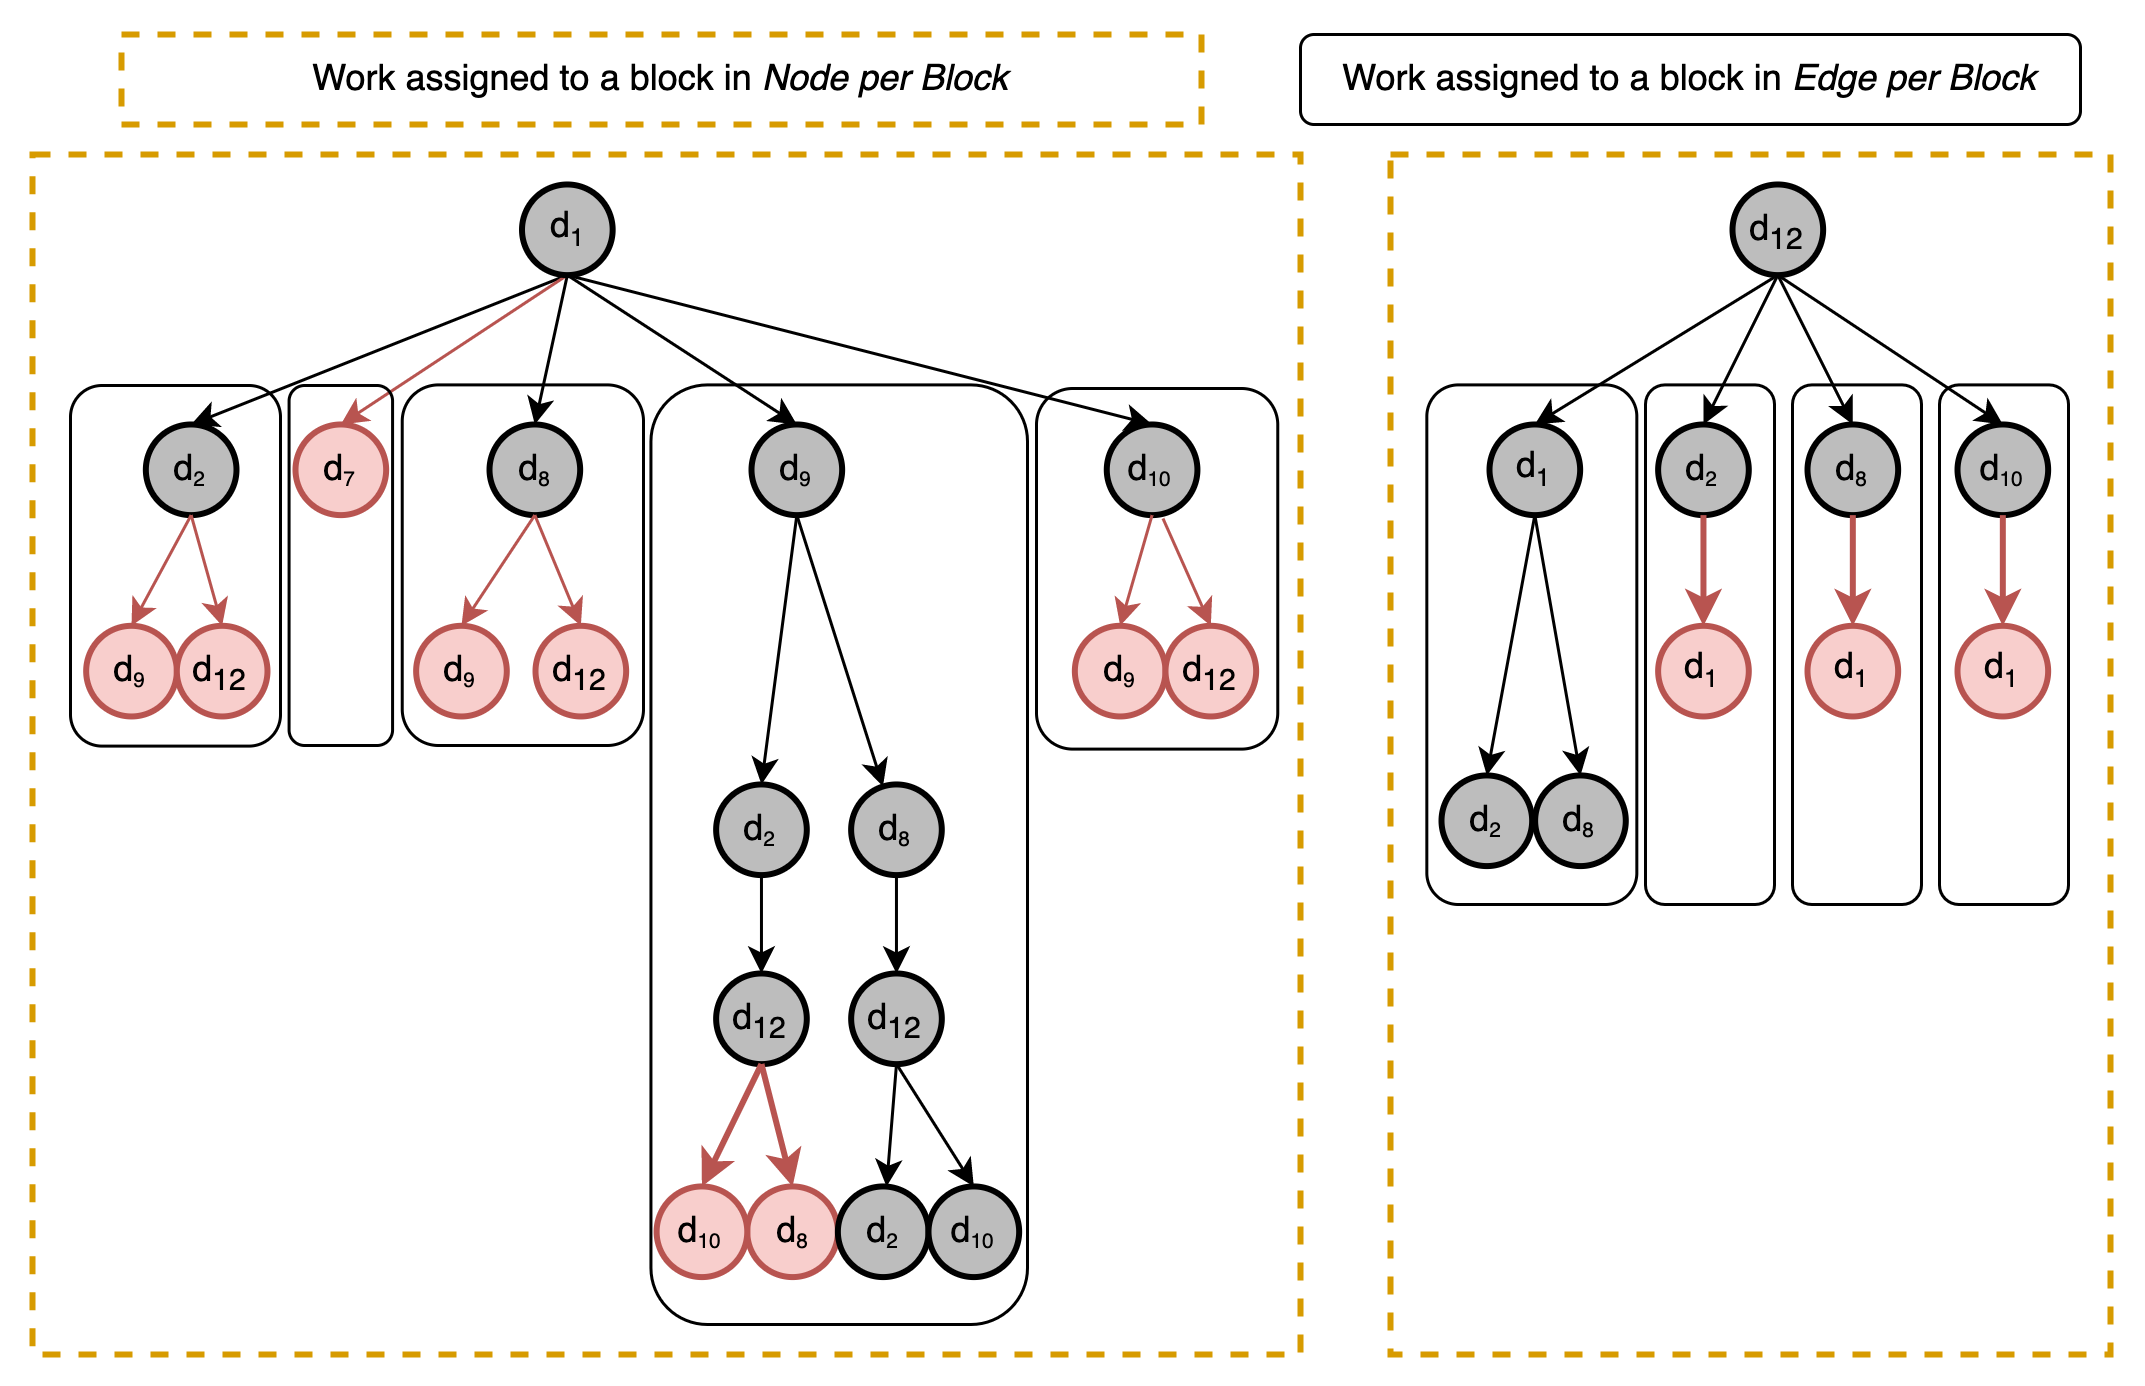
\includegraphics[width=\textwidth]{fig/parallelization-scheme.png}
    \caption{Parallelization Schemes}
    \label{fig:parallelization-schemes}
\end{figure}

Two techniques were implemented to reduce the load imbalance, (1) Task scheduling, and (2) Hybrid Parallelism.
Some runtime insights from the baseline are presented to explain these improvements, these insights also quantify the observations from baseline.
\subsubsection*{Observation 1 - Run time vs Degree}
Figure \ref{fig:runtime-vs-degree} shows the relationship between degree of the root node and runtime as a log-log plot.
It is clear that the run time is exponentially related to the root node degree also there is huge variation in the run time at same degree.
\begin{figure}
    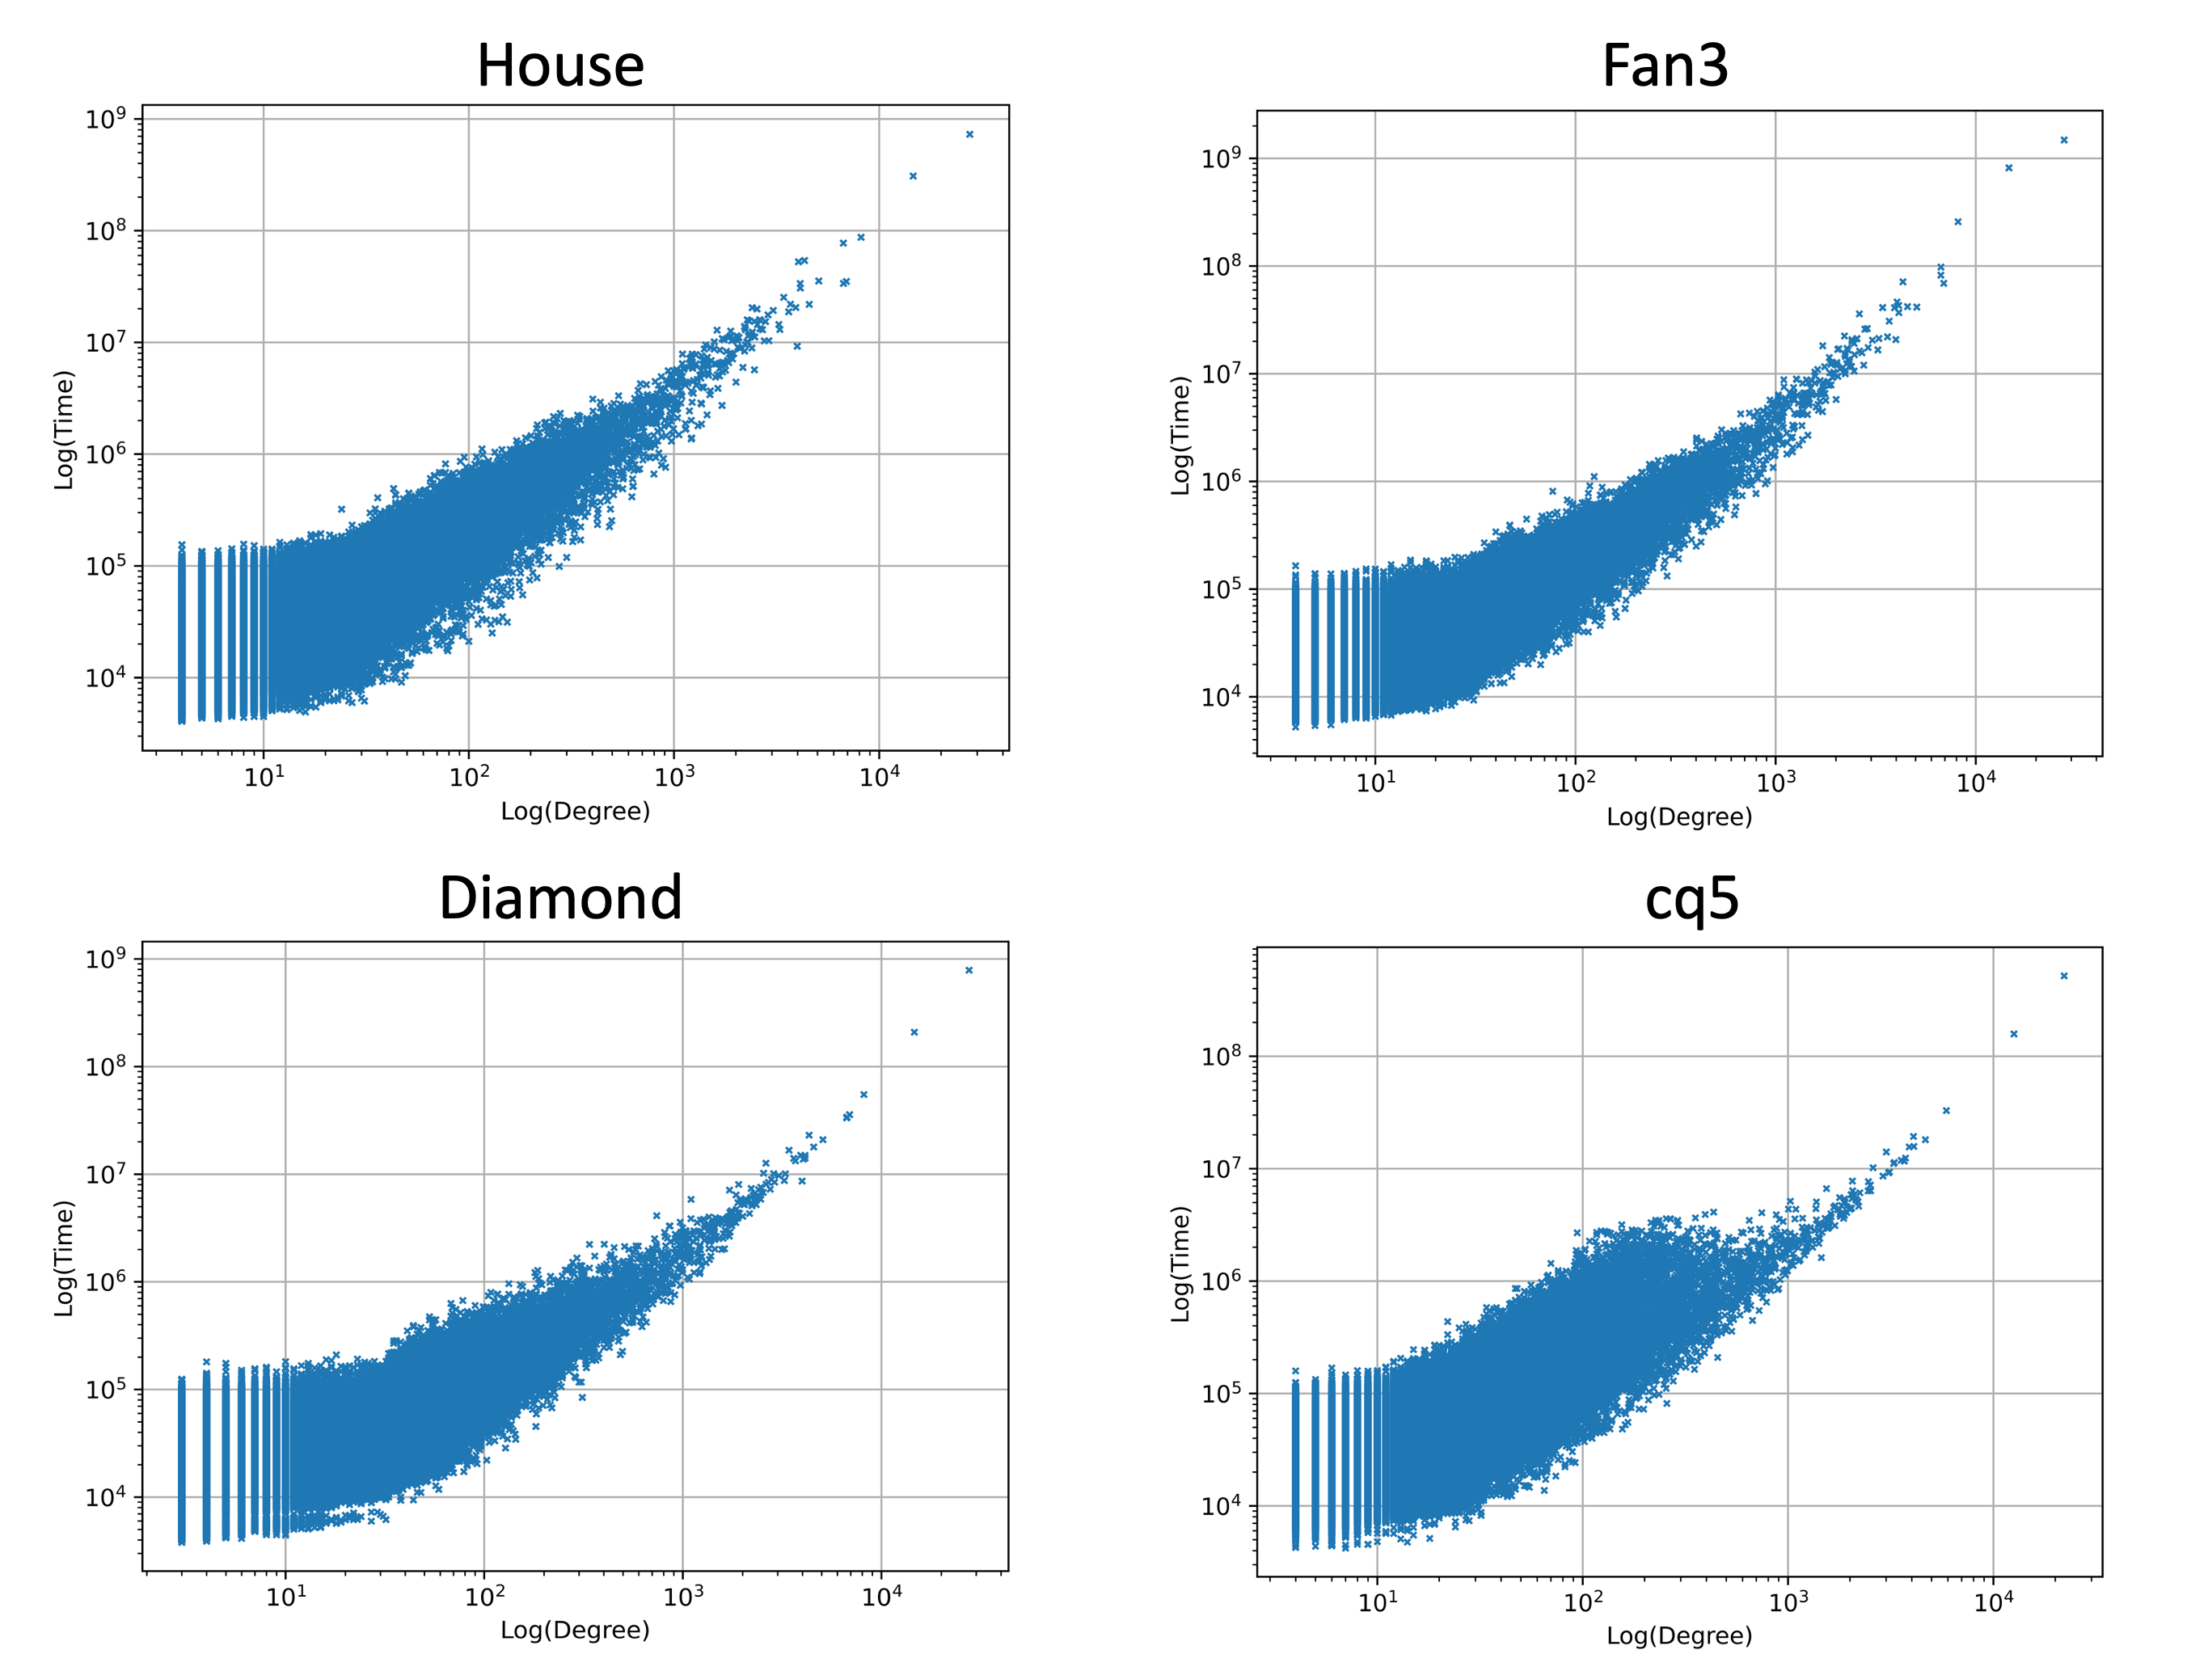
\includegraphics[width=\textwidth]{fig/improvements/time-vs-degree.png}
    \caption{Degree vs Runtime for data graph com-youtube}
    \label{fig:runtime-vs-degree}
\end{figure}

\subsubsection*{Observation 2 - Load balance comparison}
Given the trend between runtime and degree of the root node, the node per block scheme is expected to show a huge load imbalance.
The load balance is supposed to improve for edge per block scheme as it would split the work offered by a high degree root node into several blocks.
Figure \ref{fig:load-balance-baseline} shows the load balance across SMs for various query graphs as standard box plot. This is computed by finding the processing time spent by each SM during the kernel lifetime. These times are then normalized to remove variability due to query graphs. It is clear from the figure that the edge per block parallelization scheme significantly improves load balance.
\begin{figure}
    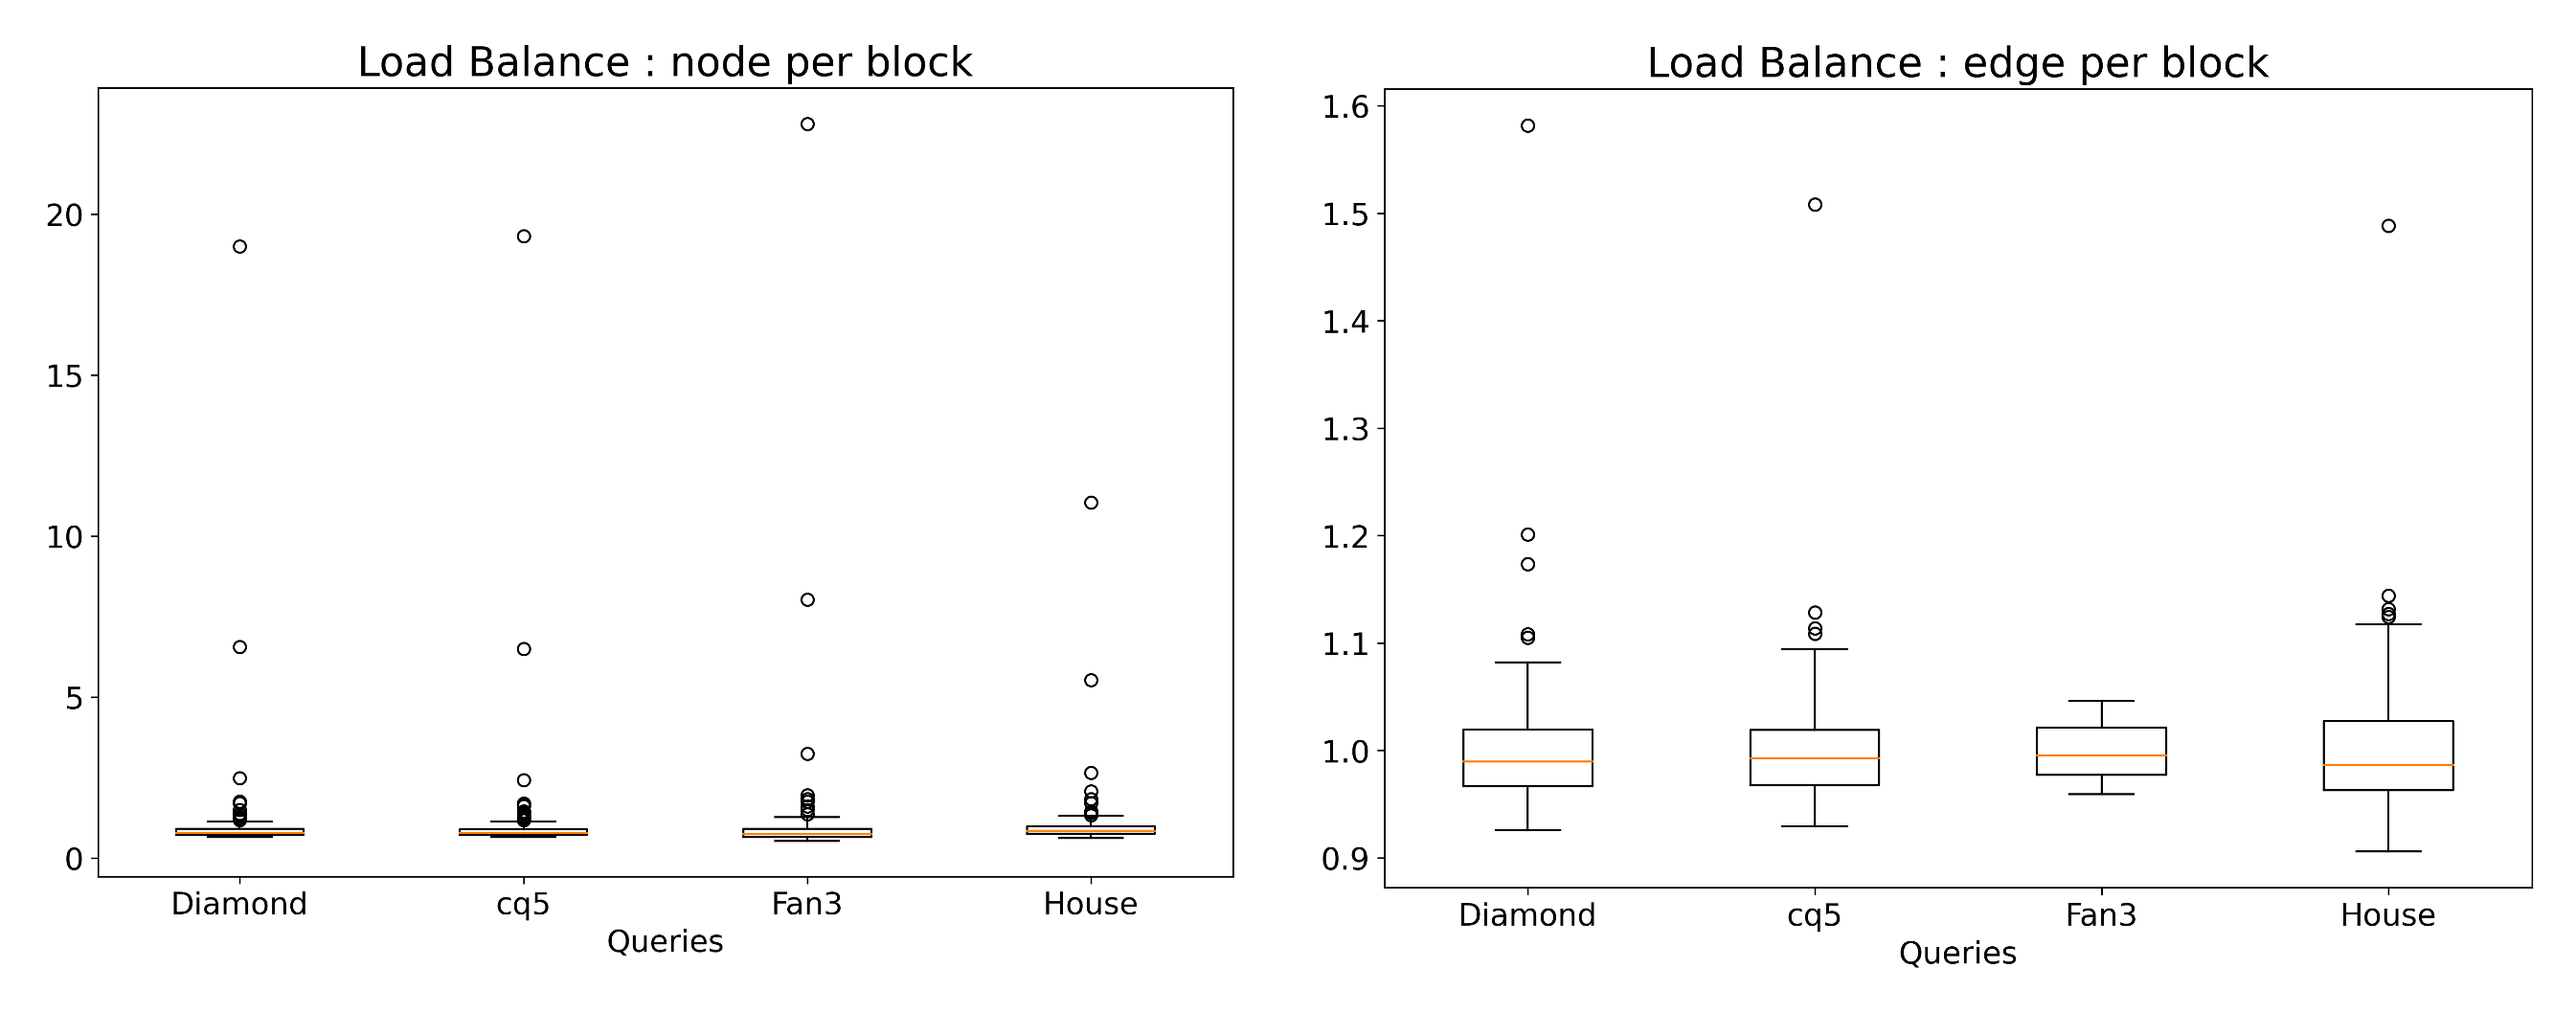
\includegraphics[width=\textwidth]{fig/improvements/yt_lb-baseline_byedge.png}
    \caption{com-youtube load balance with different parallelization schemes}
    \label{fig:load-balance-baseline}
\end{figure}

\subsubsection*{Observation 3 - Load balance for low degree nodes}
Since the trend between degree and runtime is exponential, the subtrees originating from nodes with low degrees will likely have lesser variation in run times.
Figure \ref{fig:load-balance-LD} shows there is negligible load imbalance for low degree nodes.
For these findings, all nodes with degree higher than cutoff were filtered out before kernel launch.
\begin{figure}
    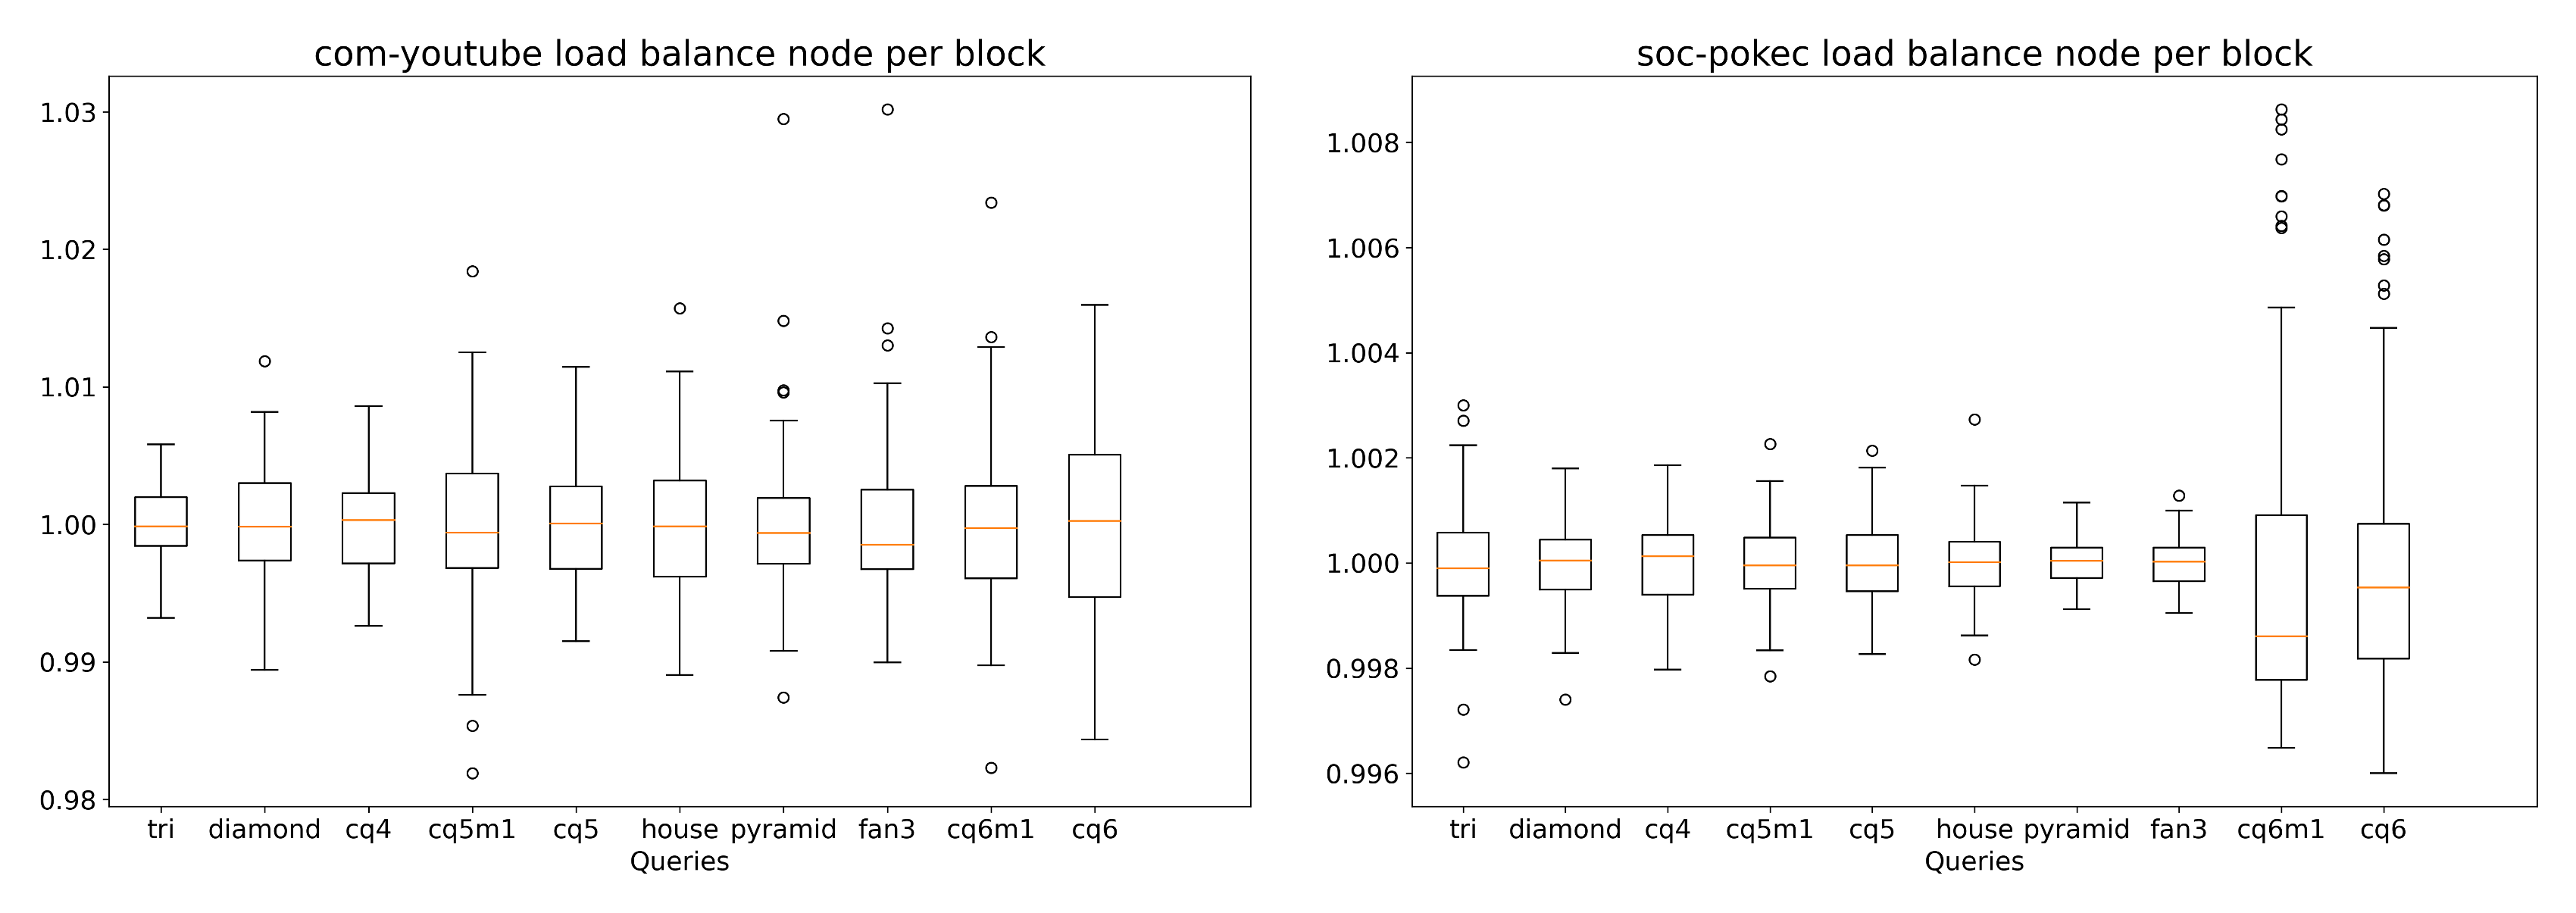
\includegraphics[width=\textwidth]{fig/improvements/load-balance-LD.png}
    \caption{Load balance for nodes with degree $\leq 256$ }
    \label{fig:load-balance-LD}
\end{figure}

The claim from the authors of \cite{PARSEC_VD} was edge per block scheme works better than node per block for queries of size greater than five.
One reason for this claim is implied by the load balance observations above, however, it does not explain the slow performance of the edge per block kernel.
The reason here is strictly based on the implementation. For the edge per block scheme in \cite{PARSEC_VD}, each block induces its subgraph. This causes extra workload hence the edge per block implementation outperforms only for larger query graphs as they exhibit worse load balance.
To remove this redundant work, the kernel is split with different parallelization schemes in each part.
The first kernel ensures non-redundancy while inducing subgraphs by using the node per block scheme.
The second kernel uses these induced subgraphs to perform search tree traversal using the edge per block scheme while ensuring better load balance.

Since the kernels are split, the persistent memory technique used in the baseline \cite{PARSEC_VD} needs to be removed.
To minimize the total number of kernel launches and better resource utilization a runtime query to the device memory is performed and the number of nodes to process at once is found accordingly.

It is clear from Figure \ref{fig:load-balance-LD} that the low degree nodes do not exhibit load imbalance with node per block parallelization. Since, splitting the kernels loses cache benefits and causes launch overheads a cutoff scheme was developed. Nodes with degree less than cutoff would perform subgraph inducing and search tree traversal in node per block fashion while nodes with degree higher than cutoff would perform these operations as mentioned above.
Figure \ref{fig:hybrid-par-speedups} shows the improvement in runtimes for the com-youtube data graph across different queries with cutoff being 2048.

\begin{figure}
    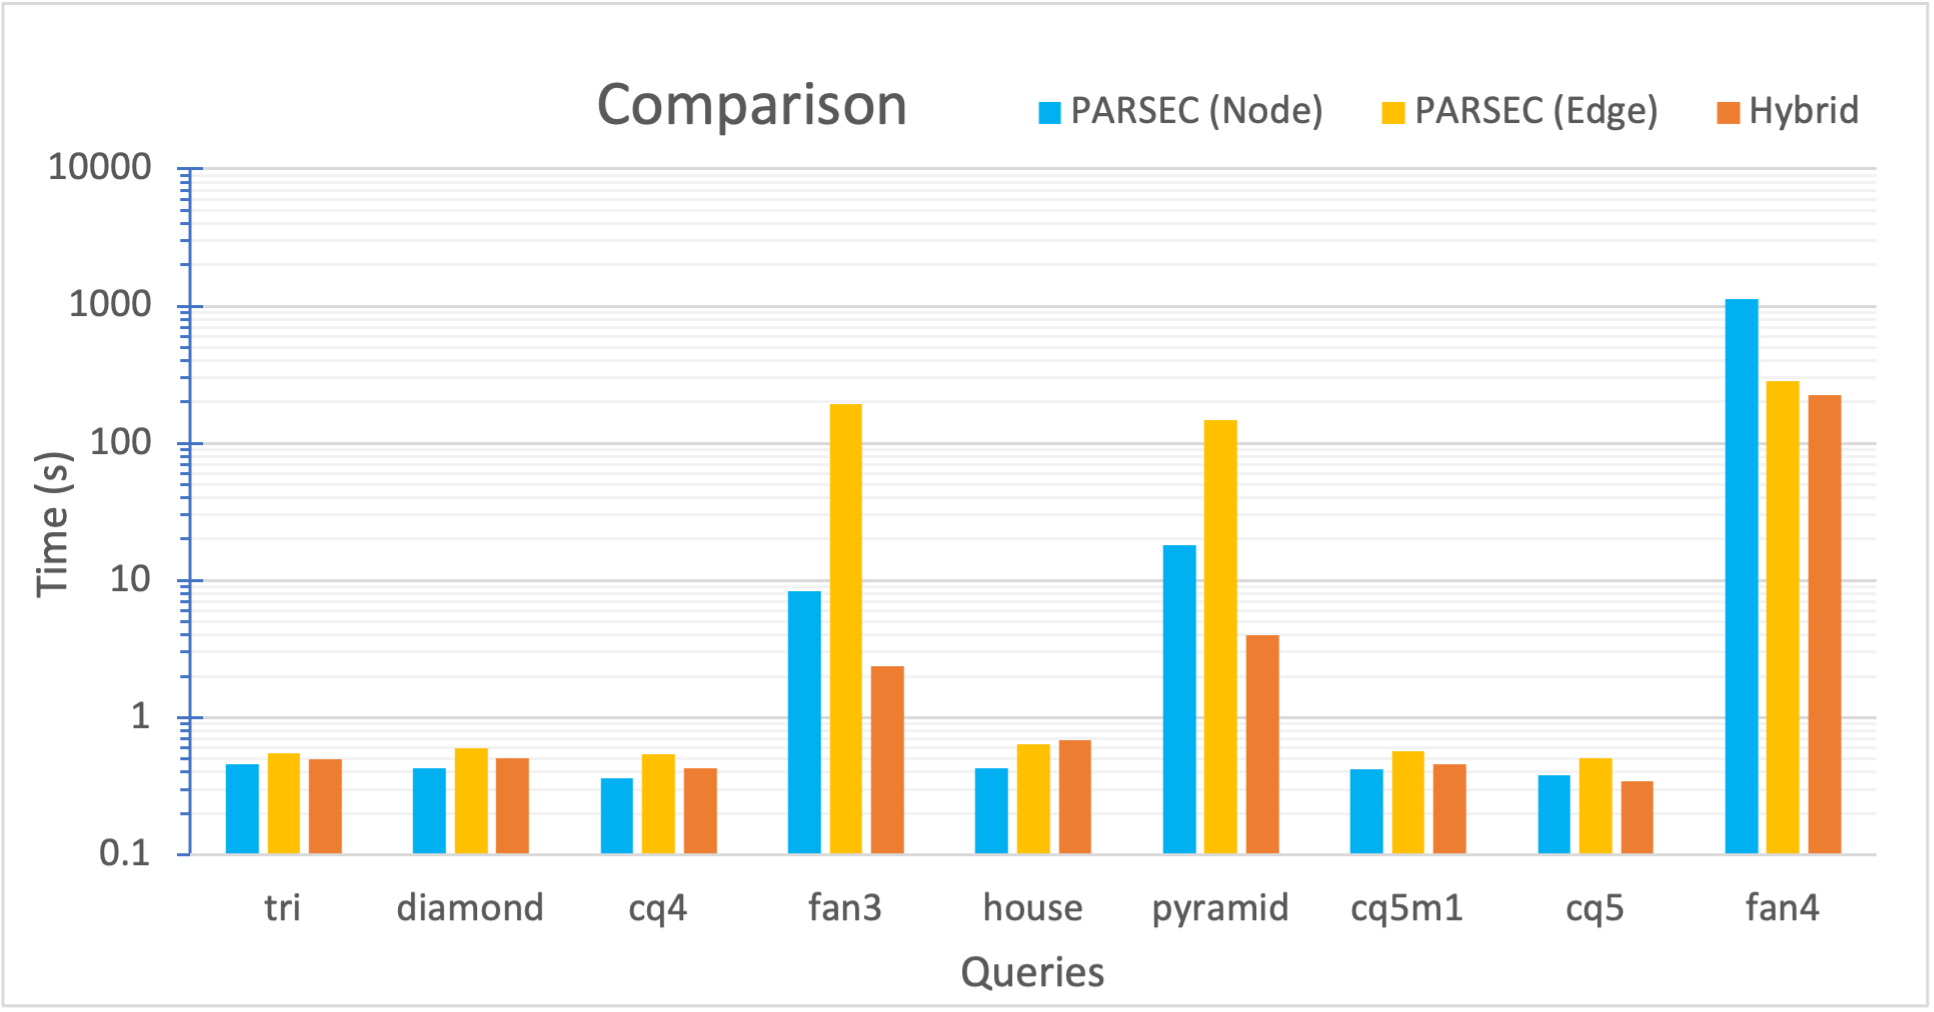
\includegraphics[width=\textwidth]{fig/improvements/Hybrid-parallelism-speedups.png}
    \caption{Run times with Hybrid parallelism for com-youtube}
    \label{fig:hybrid-par-speedups}
\end{figure}

Empirical testing was performed to fix a cutoff value across different queries.
It was found that for dense templates like \textit{cqx} and \textit{cqxm1} cutoff value between $(1024 - 2048)$ is better while for sparse templates like \textit{fans, pyramids,} and \textit{wheels} cutoff value around $768$ achieved best results.
Figure \ref{fig:cutoff-tests} shows the time fraction of runtimes across different cutoffs, time fraction is defined as runtime of an instance divided by average time across all instances (Lower is better for these Figure).
Using these insights the cutoff was decided at runtime based on input query.

\begin{figure}
    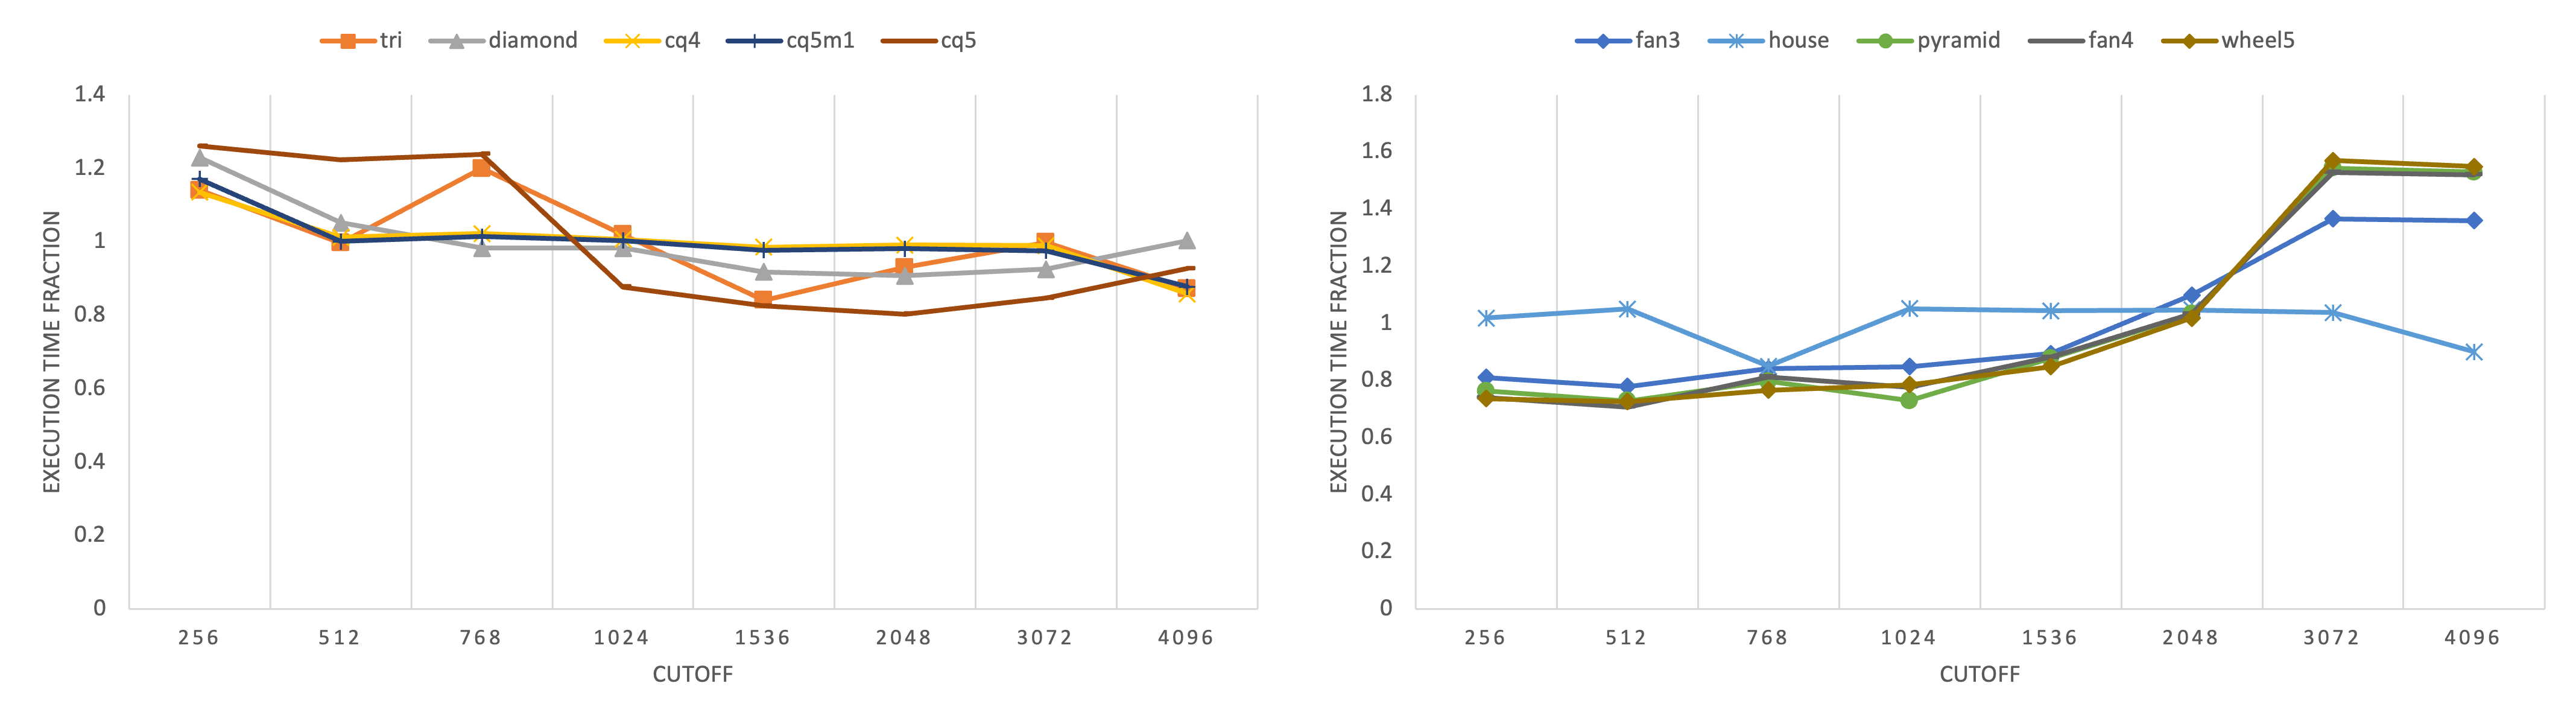
\includegraphics[width=\textwidth]{fig/improvements/cutoff-tests-yt.png}
    \caption{Run time fractions vs cutoff for com-youtube}
    \label{fig:cutoff-tests}
\end{figure}